\documentclass[12pt]{article}
\usepackage{acro}
\usepackage{amsmath}
\usepackage{amssymb}
\usepackage{amsfonts}
\usepackage{graphicx}
\usepackage{float}
\usepackage{hyperref}
\usepackage{listings}
\usepackage{color}
\usepackage{verbatim}
\usepackage{fancyvrb}
\usepackage{fancyhdr}
\usepackage[T1]{fontenc}
\usepackage{minted}


\DeclareAcronym{test}{
	short = ST,
	long = Something Test,
}
\DeclareAcronym{CI/CD}{
	short = CI/CD,
	long = Continuous Integration/Continuous Deployment,
}
\DeclareAcronym{CTF}{
	short = CTF,
	long = Capture The Flag,
}
\DeclareAcronym{CVE}{
	short = CVE,
	long = Common Vulnerabilities and Exposures,
}
\DeclareAcronym{CLI}{
	short = CLI,
	long = Command Line Interface,
}
\DeclareAcronym{API}{
	short = API,
	long = Application Programming Interface,
}
\DeclareAcronym{HTTP}{
	short = HTTP,
	long = Hyper Text Transfer Protocol,
}
\DeclareAcronym{HTTPS}{
	short = HTTPS,
	long = Hyper Text Transfer Protocol Secure,
}
\DeclareAcronym{SSH}{
	short = SSH,
	long = Secure Shell,
}
% URL - Uniform Resource Locator
\DeclareAcronym{URL}{
	short = URL,
	long = Uniform Resource Locator,
}
\DeclareAcronym{DNS}{
	short = DNS,
	long = Domain Name System,
}
\DeclareAcronym{IP}{
	short = IP,
	long = Internet Protocol,
}
\DeclareAcronym{OS}{
	short = OS,
	long = Operating System,
}
\DeclareAcronym{VM}{
	short = VM,
	long = Virtual Machine,
}
\DeclareAcronym{Git}{
	short = Git,
	long = Global Information Tracker,
}
\DeclareAcronym{RESTAPI}{
	short = REST API,
	long = Representational State Transfer Application Programming Interface,
}
\DeclareAcronym{CS}{
	short = CS,
	long = Computer Science,
}
\DeclareAcronym{devops}{
	short = DevOps,
	long = Development and Operations,
}
\DeclareAcronym{SSL}{
	short = SSL,
	long = Secure Sockets Layer,
}
% CA - Certificate Authority
\DeclareAcronym{CA}{
	short = CA,
	long = Certificate Authority,
}
% RSA - Rivest-Shamir-Adleman
\DeclareAcronym{RSA}{
	short = RSA,
	long = Rivest-Shamir-Adleman,
}
% CSR - Certificate Signing Request
\DeclareAcronym{CSR}{
	short = CSR,
	long = Certificate Signing Request,
}
% x509 - Standard for Public Key Certificates
\DeclareAcronym{x509}{
	short = x509,
	long = Standard for Public Key Certificates,
}
% NAT - Network Address Translation
\DeclareAcronym{NAT}{
	short = NAT,
	long = Network Address Translation,
}
% CN - Common Name
\DeclareAcronym{CN}{
	short = CN,
	long = Common Name,
}
% FQDN - Fully Qualified Domain Name
\DeclareAcronym{FQDN}{
	short = FQDN,
	long = Fully Qualified Domain Name,
}
% YAML - YAML Ain't Markup Language
\DeclareAcronym{YAML}{
	short = YAML,
	long = YAML Ain't Markup Language,
}
% SDK - Software Development Kit
\DeclareAcronym{SDK}{
	short = SDK,
	long = Software Development Kit,
}
% AAU - Aalborg University
\DeclareAcronym{AAU}{
	short = AAU,
	long = Aalborg University,
}
% SDU - University of Southern Denmark
\DeclareAcronym{SDU}{
	short = SDU,
	long = University of Southern Denmark,
}
% IaaS - Infrastructure as a Service
\DeclareAcronym{IaaS}{
	short = IaaS,
	long = Infrastructure as a Service,
}
% DeiC - Danish e-Infrastructure Consortium
\DeclareAcronym{DeiC}{
	short = DeiC,
	long = Danish e-Infrastructure Consortium,
}
% GCP - Google Cloud Platform
\DeclareAcronym{GCP}{
	short = GCP,
	long = Google Cloud Platform,
}
% AWS - Amazon Web Services
\DeclareAcronym{AWS}{
	short = AWS,
	long = Amazon Web Services,
}
% Azure - Microsoft Azure
\DeclareAcronym{Azure}{
	short = Azure,
	long = Microsoft Azure,
}
% vCPU - Virtual Central Processing Unit
\DeclareAcronym{vCPU}{
	short = vCPU,
	long = Virtual Central Processing Unit,
}
% RAM - Random Access Memory
\DeclareAcronym{RAM}{
	short = RAM,
	long = Random Access Memory,
}
% DDC - De Danske Cybermesterskaber
\DeclareAcronym{DDC}{
	short = DDC,
	long = De Danske Cybermesterskaber,
}
% GUAC - Apache Guacamole
\DeclareAcronym{GUAC}{
	short = GUAC,
	long = Apache Guacamole,
}
% Golang - Go Programming Language
\DeclareAcronym{Golang}{
	short = Go,
	long = Go Programming Language,
}
% RDP - Remote Desktop Protocol
\DeclareAcronym{RDP}{
	short = RDP,
	long = Remote Desktop Protocol,
}
% gRPC - gRPC Remote Procedure Call
\DeclareAcronym{gRPC}{
	short = gRPC,
	long = gRPC Remote Procedure Call,
}
% HAAUKINS - HAAUKINS
\DeclareAcronym{HAAUKINS}{
	short = \javaf{HAAUKINS},
	long = HAAUKINS,
}
% TLD - Top Level Domain
\DeclareAcronym{TLD}{
	short = TLD,
	long = Top Level Domain,
}
% CI - Continuous Integration
\DeclareAcronym{CI}{
	short = CI,
	long = Continuous Integration,
}
% CD - Continuous Deployment
\DeclareAcronym{CD}{
	short = CD,
	long = Continuous Deployment,
}
% CSV - Comma Separated Values
\DeclareAcronym{CSV}{
	short = CSV,
	long = Comma Separated Values,
}
% TOS - Terms of Service
\DeclareAcronym{TOS}{
	short = TOS,
	long = Terms of Service,
}
% Ucloud - Ucloud
\DeclareAcronym{Ucloud}{
	short = Ucloud,
	long = Ucloud,
}


\begin{document}

\printacronyms



\title{Notes}
\author{Morten}

\maketitle


\begin{itemize}
    \item First: Gitea is an open source project and is there subjective to changes at any time. For this project,
    I need to ensure that the end result is the same as when I started the project. 
    To circumvent this, the base image of Gitea is chosen to be version 1.16.5. Now why this version? 
    Based some testing it seems that most of the API admin options are unavailable in version later than 1.19.0. Version between 1.16.5 and 1.19.0
    have changes which impacts the use of admin API options.
    Using the version 1.16.5 Docker image esnure that even though long time developing this project, the base image stay the same and 
    the end result will be same as when i started the project, and when the user pulls the image.
    \item Second: The configuration of Gitea needs to be static. When Gitea is installed, it will prompt the installer of Gitea 
    to specify what that person wants. This information will be stored in a special file called app.ini. This file is 
    used by Gitea to configure itself\ref{fig:gitea_app_ini_remote}. The rest of the app.ini file for this project
    can be found the source code of the project under Gitea/app.ini.
    \item Third: Users needs to be created at initialization, so that when the user start the image via docker-compose. 
    The database is already populated with users, and the user can start using the service right away.
    This is done with python3\cite{python} script which 
    post users to the database via a \ac{RESTAPI}, with admin credentials.
\end{itemize}

cl% Create simple notes latex docus
\section{Pipeline}
For the pipeline using docker and making docker the essential part of the pipeline.
Because of the necessity of docker in the pipeline, is because the scalability of the pipeline.
Docker also make the pipeline more portable, because of the docker images, that can be used on any machine.
If I dont have the possible of deploying the pipeline directly on another machines, the use
for the project fades away.

\section{Docker}
\label{sec:docker}
Docker plays a pivotal role in this project, serving as an integral tool. 
It offers a clean and efficient means of running instances that essentially 
need to be isolated once they have completed their execution. 
This allows for the encapsulation of the machines or infrastructure used for the \ac{CTF} within Docker images, 
which can then be shared with other systems. When these images are executed on those systems, the expectation is to achieve consistent outcomes.

Before delving into the Docker specifics, it's essential to understand Docker's networking capabilities.
Docker networking simplifies various aspects of network management.
It provides a mechanism for exposing Docker containers to the external world, enabling communication between containers,
and also enforcing isolation between them. This isolation is particularly vital. For instance,
if there's a Docker container running a webserver that needs to be accessible from the outside,
Docker's networking features come into play. You can create a dedicated Docker network and connect
the webserver container to it. 
Subsequently, other Docker containers can also be linked to this network, 
allowing them to communicate internally while remaining isolated from the external world, preventing unwanted access to the webserver.
\begin{figure}
    \centering
    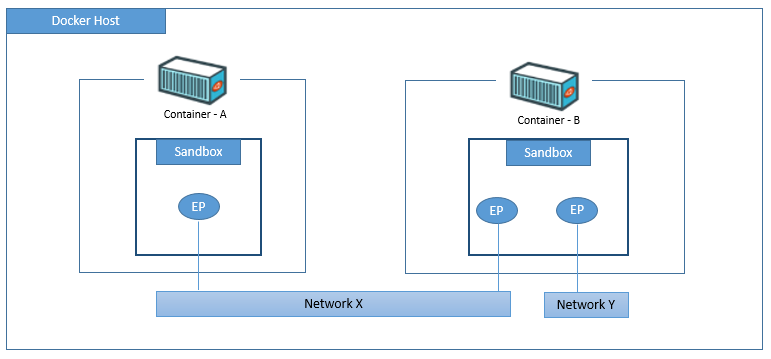
\includegraphics[width=0.8\textwidth]{images/docker_networks.png}
    \caption{Docker network}
    \label{fig:docker_network}
\end{figure}
Now as seen on the beautiful figure \ref{fig:docker_network} we have a docker network, which is called "network X".
Now as explained before every container attached to "network X" will be able to communicate with each other.
It can also talk to the outside world, but the outside can only talk to it, if I choose in my docker configuration to expose the container,
the port can be arbitrary.

Docker has a couple of different network types.
\begin{itemize}
    \item Bridge
    \item Host
    \item Overlay
    \item Macvlan
    \item None
\end{itemize}

Now I dont want to go into unnecessary details about the different network types, but I will explain the ones I have used in the project.
\subsection{Bridge}
In this project, I initially intended to utilize MacVlan,
but due to the fact that I'm running Docker on a uCloud platform where
the underlying hardware configuration seems to use IPVlan in conjunction with an external host server,
I had to resort to using a bridge. Consequently, each machine, essentially a Docker container,
behaves like a regular computer on a network. This has posed challenges because I
lack control over network-related aspects and cannot implement advanced functionalities.
The uCloud, or more specifically, the AAU-cluster network, is isolated from me. 
To perform any internal network tasks, I would need internet access, but the network restricts access
to anything other than SSH connections,
limiting my ability to carry out more advanced tasks.


\section{Drone CI/CD}

Drone\cite{droneio} is a CI/CD tool that is used to automate the process of building, testing and deploying software.
Drone is a container-native CI/CD platform built on Docker, written in Go. It uses a simple YAML configuration file,
and it leverages Docker, so it's easy to add support for new languages and frameworks.

Drone is a self-service solution that allows developers to build, test and deploy their own code.
It is designed to be easy to use, and it is built on top of Docker, so it is easy to add support for new languages and frameworks.

Also what very important about drone is that it is open source. Everything about the DroneAPI is open source and 
avaiable on their website. Now this tool seemed like the perfect tool for the job, because of the simplicity of the tool.
Running it together with gitea also seemed like a good idea, because of the integration between the two tools.
Boy was I wrong. 

\subsection{Drone problems}
\subsubsection{Problem 1, integration with gitea over OAuth2}
Other than starting out figuring out how to run drone, I had to figure out how to integrate it with gitea.
Now later version of drone, had its own database of users and therefore didn't have to rely on gitea for authentication.
Now this means that before being able to run drone runners to execute pipeline, the user that wish to use drone,
needs to authenticate with the gitea server, and post a access token to the gitea server. Essentially the user needs a token 
when is used to authenticate with the gitea server.
Now the authentication process is not a problem, the drone CI/CD documentation is very specific about how to do it and if done 
correctly it'll work fine.
Now the big problem is posting the token to the gitea server. The gitea server will not accept the token, being posted over http connection,
and it refusing the connection. 
Since drone need to make it's access token available to the gitea server, it needs to be able to post it to the gitea server.
The problem can be solved by using a proxy or a https connection on the gitea server, but that is not a viable solution.

\subsubsection{Problem 2, Advertised problem by drone}
Now the is linked to the first problem and is about the network aspect of drone.
The authentication of the user is done in the brower. WHen that is done drone obviously needs to be able to communicate with the gitea server.
Now the problem, and im not sure how docker compose works in this part, but what I've deciphered from the internet is that 
drone might not be able to find the gitea server, and post the token to it.

\subsubsection{Problem 3, Drone runner}
When the Drone server is operational, it acts as the intermediary connecting the Git server 
and the runners responsible for executing the pipeline. 
To ensure a smooth pipeline execution, it is imperative that the pipeline configuration 
for the Drone server is exceptionally detailed. This configuration should explicitly define 
crucial details such as the software used to manage the Drone server, particularly Docker if the Drone runners 
are tasked with running the pipeline within Docker containers.

Furthermore, the fact that this specification must be written in YAML introduces a 
level of dependency on YAML syntax and indentation. It's important to note that the 
specific syntax and indentation requirements can vary from one software platform to another when defining the structure of the pipeline. 
Therefore, careful attention to these details is vital to ensure accurate and effective pipeline execution.

\begin{figure}
    \begin{minted}[
        gobble=4,
        frame=single,
        linenos
      ]{yaml}
        kind: pipeline
        type: docker
        name: default
            
        steps:
        - name: backend
          image: golang
          commands:
          - go build
          - go test
            
        - name: frontend
          image: node
          commands:
          - npm install
          - npm run test
      \end{minted}
\end{figure}

\subsection{Problems with droneCI problematic}
Although the Drone CI/CD tool faced some challenges, I successfully configured it to run on the same machine as the Gitea server, 
even though the official Drone documentation doesn't recommend this approach. Furthermore, 
I managed to set up both the Drone server and Gitea within the same Docker network using Docker Compose. 
However, I encountered a significant issue that led me to reconsider Drone as a pipeline tool.

Following the authentication process using Gitea OAuth2, the Drone server requires the capability to post an access token to the Gitea database. 
This access token is crucial for the Drone server to authenticate interactions between itself and the Git server. 
Unfortunately, when the Drone server attempts to perform this operation, the Git server rejects the connection because it lacks an HTTPS connection. 
This conclusion is supported by the fact that when attempting to authenticate with `http://localhost:3000`, 
the Git server refuses the connection. However, when I connect the Drone server to a Git server running on an HTTPS connection, 
the Git server accepts the connection. The specific error is:
\begin{center}
  Post \url{"http://localhost:3000/login/oauth/access_token"}: dial tcp \url{127.0.0.1:3000}: connect: connection refused
\end{center}

Due to this limitation, the Drone server is not a viable option for our pipeline, as it 
necessitates the Git server to operate on an HTTPS connection. I would prefer the Git server 
to operate on an HTTP connection for the sake of pipeline simplicity.

I already proposed a solution and something that already has been done by is not a sustainable solution. 
Another solution which would was proposed on a blog page\cite{drone-solution-static-ip}. The solution is based of 
two things. One OAuth happens in the browers as mentioned either. Second, for the OAuth to happen, the drone 
server needs do the OAuth. But since it is exposed on localhost, it tries to authenticate with localhost ip, 
instead of the ip of the docker container. By specifying the ip of the docker container, the drone server will
be able to authenticate with the gitea server. This is not a sustainable solution, because the ip of the docker container
will change, if the docker container is restarted. This is not a viable solution, because the means that the image 
will become static and therefore might be subject to change.



\bibliographystyle{plain}
\bibliography{refs}

\end{document}